\documentclass[10pt,a4paper]{article}
\usepackage[margin=18mm]{geometry}
\usepackage[T1]{fontenc}
\usepackage{lmodern,microtype}
\usepackage{amsmath,amssymb}
\usepackage{graphicx,booktabs,tabularx,array,longtable,float,caption}
\usepackage[table]{xcolor}
\usepackage{enumitem}
\usepackage{titlesec}
\usepackage{tikz}
\usetikzlibrary{arrows.meta,positioning,calc,shapes.geometric}
\usepackage{pgfplots}
\pgfplotsset{compat=1.18}
\usepackage{csquotes}
\usepackage[colorlinks=true,linkcolor=blue!55!black,citecolor=blue!55!black,urlcolor=blue!55!black]{hyperref}
\usepackage[backend=biber,style=ieee,sorting=none,doi=true,url=false]{biblatex}
\addbibresource{references.bib}

% ---------- colours ----------
\definecolor{mpblue}{RGB}{28,63,87}
\definecolor{mpteal}{RGB}{18,118,132}
\definecolor{mpgold}{RGB}{183,110,47}
\definecolor{mplight}{RGB}{239,247,249}
\definecolor{mpcream}{RGB}{254,246,235}

% ---------- general layout ----------
\setlength{\parindent}{0pt}
\setlength{\parskip}{5pt}
\renewcommand{\arraystretch}{1.25}
\setlength{\tabcolsep}{4.5pt}
\setlength{\heavyrulewidth}{0.9pt}
\setlength{\lightrulewidth}{0.5pt}
\emergencystretch=3em
\raggedbottom
\widowpenalty=10000
\clubpenalty=10000
\setlength{\textfloatsep}{12pt plus 2pt minus 2pt}
\setlength{\intextsep}{10pt plus 2pt minus 2pt}
\setlist[enumerate]{itemsep=3pt,topsep=3pt,leftmargin=*}

% ---------- captions ----------
\captionsetup{font=small,labelfont={bf,color=mpblue},skip=7pt,justification=justified,singlelinecheck=false}

% ---------- headings ----------
\titleformat{\section}{\Large\bfseries\color{mpblue}}{\thesection}{0.7em}{}
\titleformat{\subsection}{\large\bfseries\color{mpteal!80!black}}{\thesubsection}{0.7em}{}
\titlespacing*{\section}{0pt}{16pt plus 3pt minus 2pt}{6pt plus 1pt}
\titlespacing*{\subsection}{0pt}{11pt plus 2pt minus 2pt}{4pt plus 1pt}

% ---------- table column types ----------
\newcolumntype{L}[1]{>{\raggedright\arraybackslash}p{#1}}
\newcolumntype{Y}{>{\raggedright\arraybackslash}X}

\newcommand{\MP}{microplastic}
\newcommand{\tracka}{\textbf{Track A (live boat sensing)}}
\newcommand{\trackb}{\textbf{Track B (geotagged collection + shoreline processing)}}
\title{\color{mpblue}\bfseries Microplastic Concentration Mapping in Freshwater\\[4pt]
\large Two Practical Measurement Tracks: Live Boat Monitoring and Portable Shoreline Post-processing}
\author{Year 3 Group Project -- Working background and concept-selection review}
\date{October 2026}
\begin{document}
\maketitle
\begin{abstract}
This revised background review combines the previously screened freshwater literature and a 49-method-family re-screen with the stakeholder's requirement to produce a portable, automated, two-dimensional map of microplastic (MP) concentration. Two workflows are evaluated: (A) real-time measurements from a boat and (B) geotagged water collection with rapid, self-contained processing at the shoreline. \textbf{Routine access to FTIR, Raman, or a chemistry laboratory is not assumed.} Camera-assisted particle counting, flow imaging, electrical impedance, fluorescence, polarisation, and water-quality proxies are compared by operating principle, deployment effort, specificity and evidence. A staged decision plan is proposed to distinguish \emph{suspected particle concentration} from a defensible \emph{microplastic concentration} estimate. Paper counts in this review are preliminary keyword-screening outcomes rather than demonstrated method performance.
\end{abstract}

\section{Stakeholder requirements and scope}
The stakeholder brief calls for a system that estimates microplastic concentration over a lake or river surface, produces a \emph{two-dimensional spatial concentration map}, surveys relatively large areas quickly, is practical to deploy and can be validated against appropriate reference measurements. The briefing explicitly allows direct measurement or image-based methods and a boat or aerial platform. It notes that conventional collection, filtration and microscope counting are slow and have limited spatial coverage. Here we take the boat as the vehicle and reformulate measurement into two feasible deployment tracks. \textbf{A continuous coloured image of water appearance is not, by itself, a validated map of microplastic concentration.} Similarly, GPS only places estimates on a map; it does not establish that they represent plastic particles \cite{Chen2021,Chen2023,Blevins2021}.

The current engineering constraint is that \textbf{routine specialist laboratory access is impractical}. This makes a compact, cleanable, low-maintenance measurement path and a robust portable cross-check especially important. Low-cost field processing can support preliminary concentration estimates, while polymer-specific identification would still need occasional external testing if definitive MP attribution is required.

\subsection{What is meant by concentration?}
For counted particles, the target quantity is $C=N_{\mathrm{MP}}/V_{\mathrm{water}}$ in particles/L, stated for a defined detectable particle-size range and sampling depth. A count of \emph{suspected} MPs inferred from images should be reported as such until specificity has been demonstrated. For model-derived estimates, uncertainty and calibration domain must be reported. Polymer mass concentrations from thermal analysis are a different measurand and cannot simply be substituted for particles/L \cite{Blevins2021,Sefiloglu2024}.

\section{Literature selection and four background themes}
From the prior Web of Science--Scopus search, 18,942 records were identified. After removing 7,318 duplicates and 727 document-type exclusions, 10,897 remained for title/abstract screening; 10,833 were preliminary include candidates and 64 needed manual review. The four theme tags overlap: causes (6,430), water effects (7,575), laboratory/measurement methods (6,654) and data trends/mapping (5,320). These labels do not represent completed full-text eligibility screening.

\begin{figure}[H]\centering
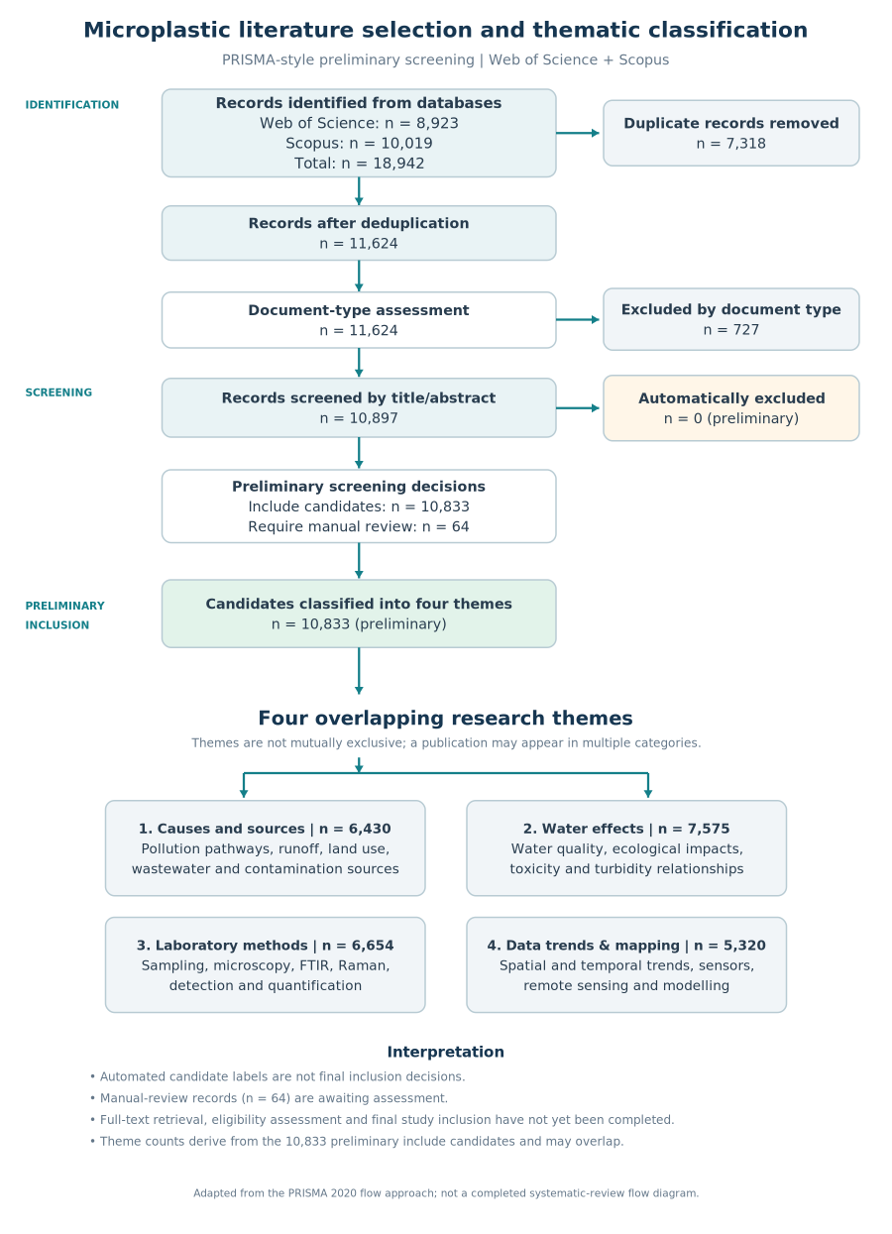
\includegraphics[height=0.55\textheight,width=\linewidth,keepaspectratio]{Figures/prisma.png}
\caption{Original preliminary screening and four overlapping classifications. Counts are not independent study totals.}\label{fig:prisma}
\end{figure}

\subsection{Sources and causes of riverborne microplastics}
Land use, wastewater, roads, runoff and local discharge influence the spatial distribution of MPs. Tropical river studies illustrate variation between sites and sampling periods rather than one uniform concentration across a catchment \cite{Chen2021,Chen2022,MPWE00007,MPWE00013}. For either track, each measurement must retain sampling location, date, depth and nearby environmental context.

\subsection{Effects and physical/chemical water properties}
Relevant literature covers ecological effects and associations with turbidity, conductivity, suspended solids and nutrients. These properties may influence sensor signals but are \emph{not uniquely attributable to MPs}. For instance, nitrogen/conductivity relationships in surface-water research do not demonstrate a universal electrical MP concentration sensor \cite{MPWE00002,MPWE02100}. Therefore sediment, algae, bubbles, dissolved salts and changing illumination must be tested explicitly as interferents.

\subsection{Measurement and reference methods}
Collection, filtration, microscope imaging, FTIR and Raman feature prominently in the initial screening. Image-based counting can quantify visible particles after appropriate segmentation, whereas spectroscopy can support polymer identity but requires equipment beyond the present project constraint \cite{Ermolin2024,Lee2022,UrbanCNN2024,MPWE00012}. Portable microscope imaging is therefore a feasible preliminary \emph{field-reference} for particle counts, but not a definitive chemical reference for all MPs.

\subsection{Data trends and spatial prediction}
Rivers change with rainfall, flow and location, so isolated point measurements must be mapped with times and uncertainty. Remote imagery and GIS have been explored, but translating visible surface patterns or turbidity into MP particles/L requires paired calibration and external testing \cite{Chen2021,MPWE04211,MPWE02100}. \emph{Track B can create a post-survey heat map from discrete geotagged samples; a heat map does not require that concentrations were measured while the boat was moving.}

\section{Two-track system architecture}
\subsection{Two processes, one map specification}
Figure~\ref{fig:tracks} presents two end-to-end workflows. The diagram is intentionally technology-agnostic: its purpose is to define the operational stages and thereby the criteria used to filter candidate sensing methodologies. The boat and GPS path are shared, but the sensing stage and the downstream handling occur in different places. Track A is more automated and ambitious; Track B is a practical alternative when continuous in-water particle detection is unreliable, too expensive or difficult to maintain.

\begin{figure}[H]\centering
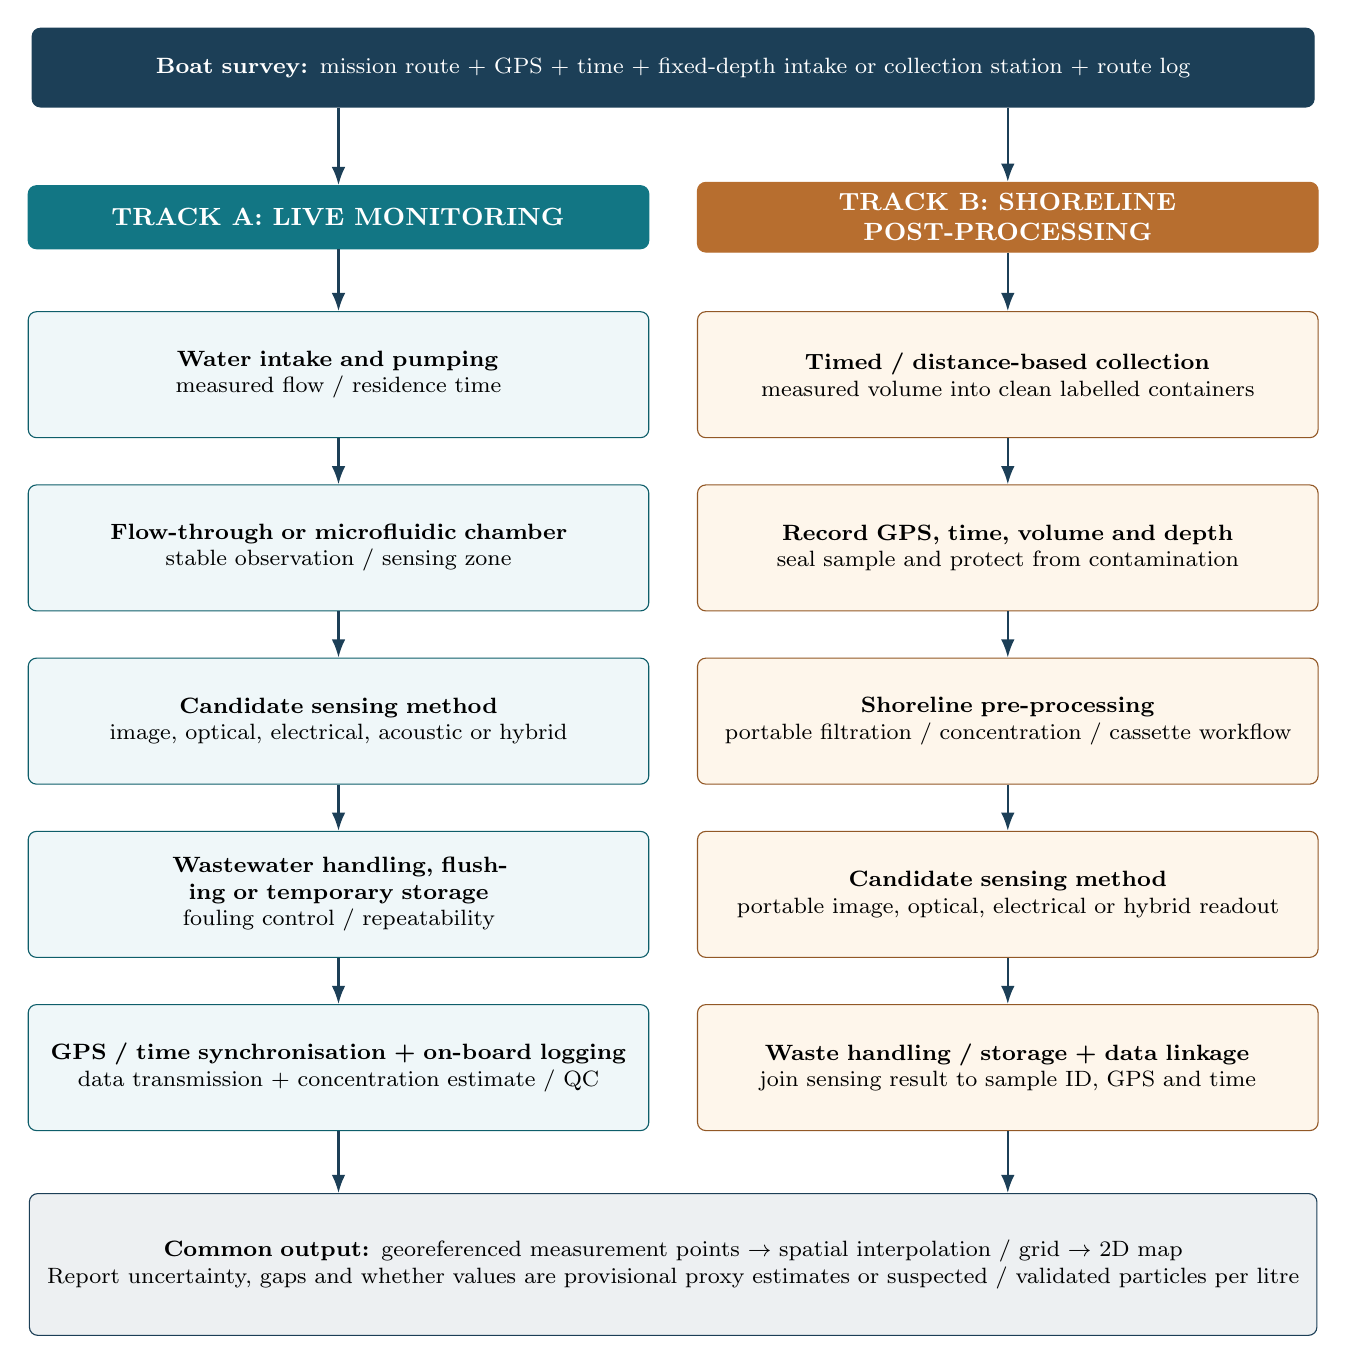
\begin{tikzpicture}[>=Latex, font=\footnotesize,
 startbox/.style={draw=mpblue,fill=mpblue,text=white,rounded corners=3pt,
   align=center,text width=16cm,minimum height=10mm,inner sep=4pt},
 hdrA/.style={draw=mpteal,fill=mpteal,text=white,rounded corners=3pt,
   align=center,text width=7.6cm,minimum height=8mm,font=\bfseries\small,inner sep=4pt},
 hdrB/.style={draw=mpgold,fill=mpgold,text=white,rounded corners=3pt,
   align=center,text width=7.6cm,minimum height=8mm,font=\bfseries\small,inner sep=4pt},
 stepA/.style={draw=mpteal!80!black,fill=mplight,rounded corners=3pt,
   align=center,text width=7.6cm,minimum height=16mm,inner sep=4pt},
 stepB/.style={draw=mpgold!80!black,fill=mpcream,rounded corners=3pt,
   align=center,text width=7.6cm,minimum height=16mm,inner sep=4pt},
 endbox/.style={draw=mpblue,fill=mpblue!8,rounded corners=3pt,
   align=center,text width=16cm,minimum height=18mm,inner sep=5pt},
 arr/.style={-Latex,thick,draw=mpblue}]

 % ---- shared start ----
 \node[startbox] (start) at (0,0)
   {\textbf{Boat survey:} mission route + GPS + time + fixed-depth intake or collection station + route log};

 % ---- track headers ----
 \node[hdrA] (hA) at (-4.25,-1.9) {TRACK A: LIVE MONITORING};
 \node[hdrB] (hB) at ( 4.25,-1.9) {TRACK B: SHORELINE POST-PROCESSING};

 % ---- Track A ----
 \node[stepA] (a1) at (-4.25,-3.9)  {\textbf{Water intake and pumping}\\ measured flow / residence time};
 \node[stepA] (a2) at (-4.25,-6.1)  {\textbf{Flow-through or microfluidic chamber}\\ stable observation / sensing zone};
 \node[stepA] (a3) at (-4.25,-8.3)  {\textbf{Candidate sensing method}\\ image, optical, electrical, acoustic or hybrid};
 \node[stepA] (a4) at (-4.25,-10.5) {\textbf{Wastewater handling, flushing or temporary storage}\\ fouling control / repeatability};
 \node[stepA] (a5) at (-4.25,-12.7) {\textbf{GPS / time synchronisation + on-board logging}\\ data transmission + concentration estimate / QC};

 % ---- Track B ----
 \node[stepB] (b1) at (4.25,-3.9)  {\textbf{Timed / distance-based collection}\\ measured volume into clean labelled containers};
 \node[stepB] (b2) at (4.25,-6.1)  {\textbf{Record GPS, time, volume and depth}\\ seal sample and protect from contamination};
 \node[stepB] (b3) at (4.25,-8.3)  {\textbf{Shoreline pre-processing}\\ portable filtration / concentration / cassette workflow};
 \node[stepB] (b4) at (4.25,-10.5) {\textbf{Candidate sensing method}\\ portable image, optical, electrical or hybrid readout};
 \node[stepB] (b5) at (4.25,-12.7) {\textbf{Waste handling / storage + data linkage}\\ join sensing result to sample ID, GPS and time};

 % ---- common output ----
 \node[endbox] (end) at (0,-15.2)
   {\textbf{Common output:} georeferenced measurement points $\rightarrow$ spatial interpolation / grid $\rightarrow$ 2D map\\
    Report uncertainty, gaps and whether values are provisional proxy estimates or suspected / validated particles per litre};

 % ---- arrows (all straight, none crossing text) ----
 \draw[arr] (start.south -| hA.north) -- (hA.north);
 \draw[arr] (start.south -| hB.north) -- (hB.north);
 \draw[arr] (hA.south) -- (a1.north);
 \draw[arr] (hB.south) -- (b1.north);
 \foreach \u/\v in {a1/a2,a2/a3,a3/a4,a4/a5,b1/b2,b2/b3,b3/b4,b4/b5}
   \draw[arr] (\u.south) -- (\v.north);
 \draw[arr] (a5.south) -- (a5.south |- end.north);
 \draw[arr] (b5.south) -- (b5.south |- end.north);
\end{tikzpicture}
\caption{Two deployable tracks that meet the briefing's mapping goal without assuming a specific sensing technology. The ``candidate sensing method'' box is the screening stage at which methods are filtered against portability, automation, contamination control, throughput, interpretability and map-readiness. Track B is batch/near-real-time after retrieval, not continuous in-situ sensing.}\label{fig:tracks}
\end{figure}

The flowchart is therefore a \emph{method-selection framework}. A sensing method should only be retained if it fits the required stage in the workflow and satisfies the briefing's constraints: portability, sufficiently rapid surveying, a defensible relationship to actual MP concentration, manageable contamination control, and practical linkage to GPS-referenced map generation \cite{ProjectBrief2026}. In the sections below, the literature is reviewed using these process requirements rather than assuming from the outset that any single technique (for example camera + AI or EIS) must be adopted.

\subsection{Track A: live monitoring from the boat}
A pump draws a measured stream through a cleanable observation channel. A fixed-focus camera and controlled LED illumination acquire frames at a known effective observed volume; segmentation and tracking distinguish successive particles from repeat appearances. GPS position should be assigned to the \emph{time the water entered the intake}, correcting for tubing/flow delay. The output can be updated at short intervals while the boat moves. Camera systems are supported by microscope-image AI and micro-flow imaging literature, though performance in untreated, moving, turbid river water is not guaranteed \cite{Lee2022,Microflow2023,UrbanCNN2024}.

\textbf{Optional adjunct:} multi-frequency impedance or polarised scattering may add non-image features, but neither resolves chemical identity automatically. Bulk water conductivity should not be labelled ``MP concentration'' without an independently validated model \cite{Blevins2021,Kim2024,Warraich2025,Polarized2021}.

\subsection{Track B: automatic collection and portable shoreline processing}
At predetermined locations or distances the boat collects a \emph{known} volume in a labelled, low-contamination sample container. Back at the shoreline, each sample is filtered on a portable membrane or processed in a sealed cassette, then imaged with a USB/digital microscope. An AI counter produces a count, and an operator reviews borderline particles and blanks. Pre-treatment or Nile Red staining is an optional method-development branch, not a necessary routine step: staining, rinsing, imaging filters and waste management must be considered \cite{ErniCassola2017,Minor2023,Zhang2023,Lee2022}. This route decouples sampling from difficult live optics and permits re-counting archived images.

\subsection{Common mapping software and quality requirements}
Both tracks store the same minimum fields: sample ID, latitude/longitude, intake time, actual water volume, sampling depth, particle-size cutoff, device model/version, quality flags and concentration estimate. A point/segment map should be shown before interpolation. If interpolation is used, choose a declared method (e.g., inverse-distance weighting or kriging if data support it), retain actual sampled points and assess its error against withheld points. A smooth heat map does not imply unsampled regions have been measured.

\section{Literature review organised around the process and screening evidence}
\subsection{What methods have actually been investigated?}
The broad Laboratory Methods keyword screen comprises 6,654 candidate records; its 14 labels describe \emph{mentions} rather than verified instrument deployment. Figure~\ref{fig:broad} shows the complete distribution. Here, those methods are interpreted against the workflow stages in Fig.~\ref{fig:tracks}: intake and chamber compatibility, sensing principle, waste/storage needs, data-linkage demands and readiness for rapid mapping. The chart therefore helps narrow which methods deserve further consideration, rather than prescribing a single sensor in advance.

\begin{figure}[H]\centering
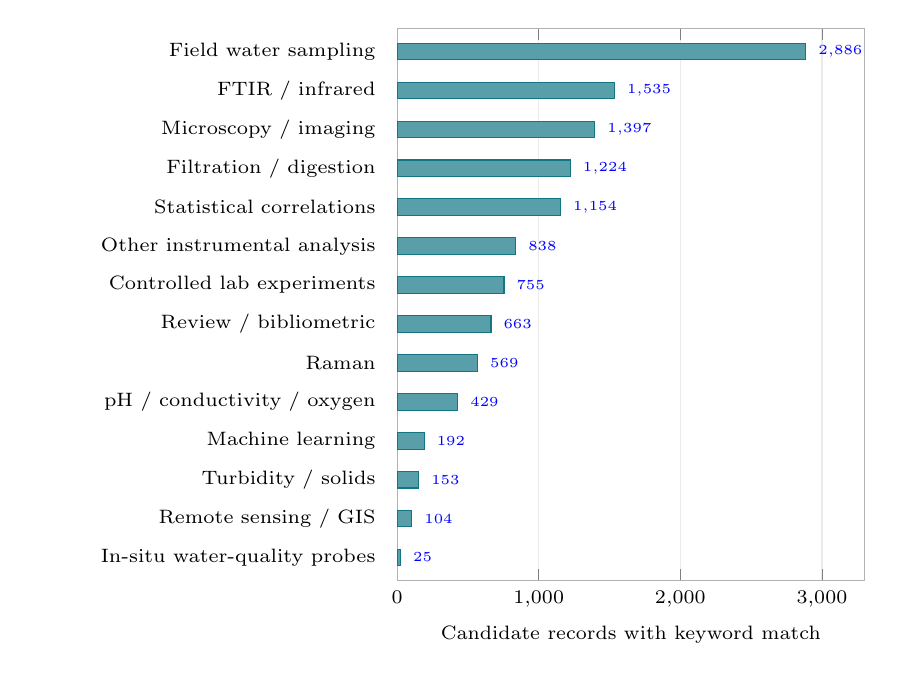
\begin{tikzpicture}
\begin{axis}[xbar,width=.62\linewidth,height=8.6cm,xmin=0,xmax=3300,ymin=-.6,ymax=13.6,
 ytick={0,...,13},
 yticklabels={{In-situ water-quality probes},{Remote sensing / GIS},{Turbidity / solids},{Machine learning},{pH / conductivity / oxygen},{Raman},{Review / bibliometric},{Controlled lab experiments},{Other instrumental analysis},{Statistical correlations},{Filtration / digestion},{Microscopy / imaging},{FTIR / infrared},{Field water sampling}},
 yticklabel style={font=\scriptsize,align=right,text width=4.3cm},tick label style={font=\scriptsize},
 ytick style={draw=none},axis line style={gray!60},clip=false,
 xlabel={Candidate records with keyword match},xlabel style={font=\scriptsize},
 xmajorgrids=true,grid style={gray!16},bar width=6pt,
 nodes near coords,point meta=x,every node near coord/.append style={font=\tiny,anchor=west,xshift=1pt}]
\addplot+[draw=mpteal,fill=mpteal!70] coordinates {(25,0)(104,1)(153,2)(192,3)(429,4)(569,5)(663,6)(755,7)(838,8)(1154,9)(1224,10)(1397,11)(1535,12)(2886,13)};
\end{axis}\end{tikzpicture}
\caption{Original 14-category method screen ($n=6{,}654$): overlapping title/abstract matches, not confirmed experimental application or accuracy.}\label{fig:broad}
\end{figure}

\subsection{Targeted sensing and processing technologies}
A complementary search across all 10,833 candidates (title/abstract/keyword fields) found relatively few mentions of impedance/EIS (5), microfluidics (22), holography (13) and polarimetric scattering (3), compared with electrochemical sensing (55), Nile Red (138) and FTIR (1,909). Ultrasound/sonication (42) includes sample preparation; these 42 are \emph{not} 42 ultrasonic MP counters. Figure~\ref{fig:targeted} keeps this screen separate from the broader 6,654-record method classification.

\begin{figure}[H]\centering
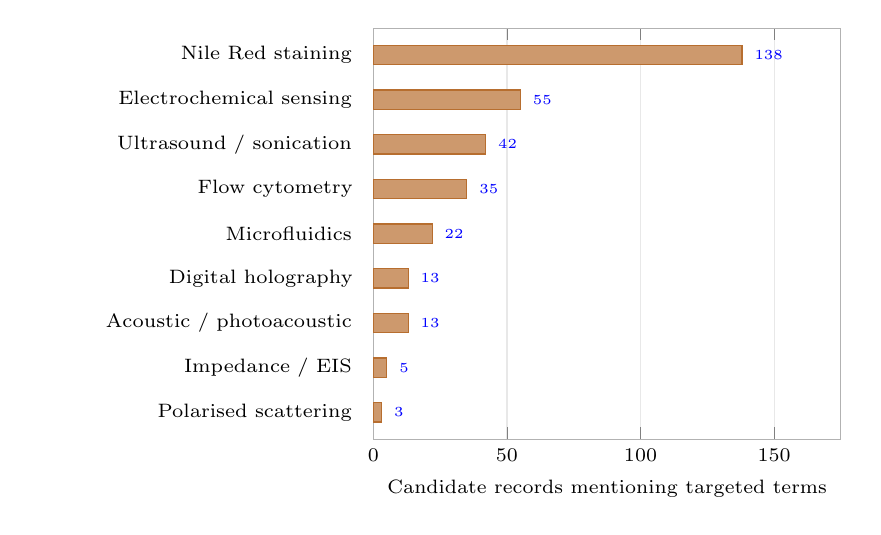
\begin{tikzpicture}
\begin{axis}[xbar,width=.62\linewidth,height=6.8cm,xmin=0,xmax=175,ytick={0,...,8},
 yticklabels={{Polarised scattering},{Impedance / EIS},{Acoustic / photoacoustic},{Digital holography},{Microfluidics},{Flow cytometry},{Ultrasound / sonication},{Electrochemical sensing},{Nile Red staining}},
 ymin=-.6,ymax=8.6,yticklabel style={font=\scriptsize,align=right,text width=4cm},tick label style={font=\scriptsize},
 ytick style={draw=none},axis line style={gray!60},clip=false,
 xlabel={Candidate records mentioning targeted terms},xlabel style={font=\scriptsize},xmajorgrids=true,grid style={gray!18},
 nodes near coords,point meta=x,every node near coord/.append style={font=\tiny,anchor=west,xshift=1pt},bar width=7pt]
\addplot+[draw=mpgold,fill=mpgold!70] coordinates {(3,0)(5,1)(13,2)(13,3)(22,4)(35,5)(42,6)(55,7)(138,8)};
\end{axis}\end{tikzpicture}
\caption{Targeted method vocabulary in 10,833 preliminary candidates; overlap and non-detection uses are possible.}\label{fig:targeted}
\end{figure}


% \clearpage
\section{Reproducible identification, filtering and elimination of sensing methodologies}
\label{sec:formal_selection}
\subsection{Scope and definition of an eligible sensor}
For reproducibility, we re-ran a new, purpose-built, multi-label search on the \textbf{10,833 original preliminary include candidates}, scanning title, abstract, author keywords and Keywords Plus (where present). The companion Python script records each regular-expression rule, its frequency, and the titles/DOIs of all matching publications. The inventory contains \textbf{49 explicitly defined method terms} in five families; no method is assumed to be experimentally deployed simply because the term occurs. These revised rules are narrower than some earlier broad-screen rules; hence the new frequencies are \textbf{not directly interchangeable} with the original 14-category counts, even when labels sound similar.

The second distinction is functional rather than bibliometric: \emph{collection/preparation}, \emph{direct or particle-related readout}, \emph{specialist reference analysis}, \emph{non-specific water-quality proxy}, and \emph{data processing/mapping} play different roles. A filter, a particle concentrator and a GIS algorithm may be essential components of a useful system, but \textbf{none is a stand-alone MP concentration sensor}. Laboratory reference methods can remain informative literature even if specialist instruments cannot be included as routine field equipment \cite{Blevins2021,Ermolin2024,Sefiloglu2024}.

\subsection{Screening funnel and disposition accounting}
\begin{figure}[H]\centering
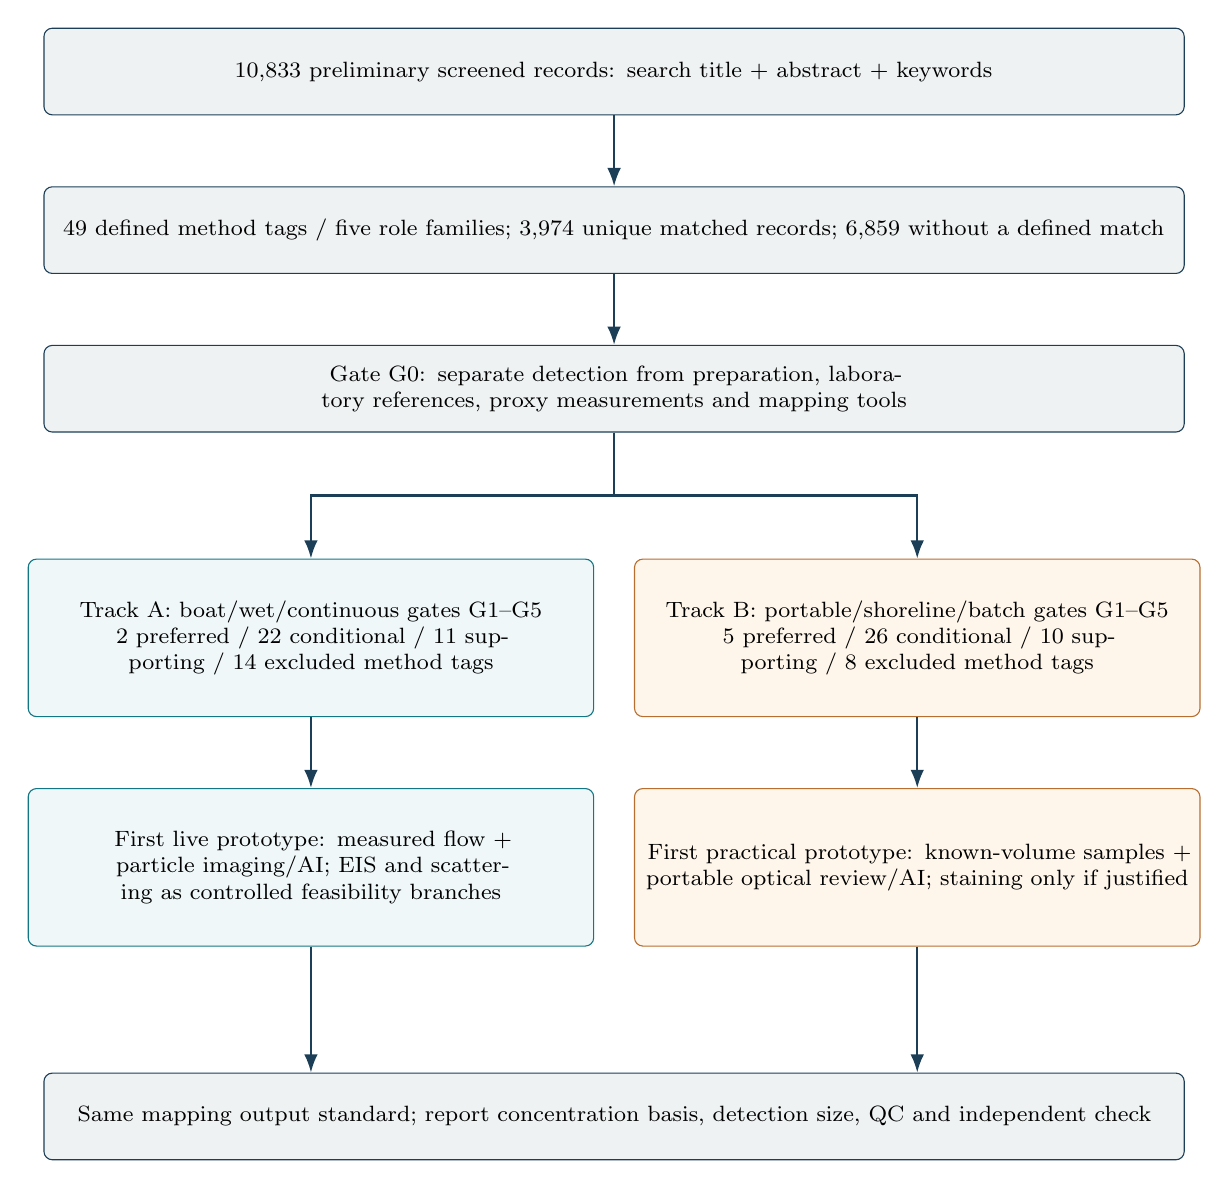
\begin{tikzpicture}[>=Latex,font=\footnotesize,
 top/.style={draw=mpblue,fill=mpblue!7,align=center,rounded corners=3pt,text width=14.2cm,minimum height=11mm,inner sep=4pt},
 aa/.style={draw=mpteal,fill=mplight,align=center,rounded corners=3pt,text width=6.9cm,minimum height=20mm,inner sep=4pt},
 bb/.style={draw=mpgold,fill=mpcream,align=center,rounded corners=3pt,text width=6.9cm,minimum height=20mm,inner sep=4pt},
 ar/.style={-Latex,thick,draw=mpblue}]
\node[top] (all) at (0,0) {10,833 preliminary screened records: search title + abstract + keywords};
\node[top,below=9mm of all] (inventory) {49 defined method tags / five role families; 3,974 unique matched records; 6,859 without a defined match};
\node[top,below=9mm of inventory] (role) {Gate G0: separate detection from preparation, laboratory references, proxy measurements and mapping tools};
\node[aa,anchor=north] (A) at ($(role.south)+(-3.85,-1.6)$) {Track A: boat/wet/continuous gates G1--G5\\2 preferred / 22 conditional / 11 supporting / 14 excluded method tags};
\node[bb,anchor=north] (B) at ($(role.south)+(3.85,-1.6)$) {Track B: portable/shoreline/batch gates G1--G5\\5 preferred / 26 conditional / 10 supporting / 8 excluded method tags};
\node[aa,below=9mm of A] (outA) {First live prototype: measured flow + particle imaging/AI; EIS and scattering as controlled feasibility branches};
\node[bb,below=9mm of B] (outB) {First practical prototype: known-volume samples + portable optical review/AI; staining only if justified};
\node[top,anchor=north] (final) at ($(outA.south)!0.5!(outB.south)+(0,-1.6)$) {Same mapping output standard; report concentration basis, detection size, QC and independent check};
\draw[ar] (all)--(inventory);
\draw[ar] (inventory)--(role);
\draw[ar] (role.south) -- ++(0,-0.8) -| (A.north);
\draw[ar] (role.south) -- ++(0,-0.8) -| (B.north);
\draw[ar] (A)--(outA);
\draw[ar] (B)--(outB);
\draw[ar] (outA.south) -- (outA.south |- final.north);
\draw[ar] (outB.south) -- (outB.south |- final.north);
\end{tikzpicture}
\caption{Reproducible method term screen followed by engineering gates; disposition counts refer to \emph{method tags}, not distinct papers or fully validated sensing devices. Unmatched records remain accessible for further screening.}\label{fig:method-funnel}
\end{figure}

\subsection{Sequential gates, rather than popularity-based selection}
\begin{table}[H]\centering\footnotesize
\caption{Method-elimination stages derived from the stakeholder specification. The criteria are testable design gates, not published accuracy thresholds.}\label{tab:selection_gates}
\begin{tabularx}{\linewidth}{@{}L{0.95cm}L{2.7cm}YY@{}}\toprule
\rowcolor{mpblue!12}\textbf{Gate} & \textbf{Main question} & \textbf{Track A: live boat} & \textbf{Track B: shoreline post-processing} \\\midrule
G0 & Is the technique a sensing output? & Differentiate detector from pump, filter, separator or prediction software. & Same distinction; standalone reference tools are allowed as components.\\
G1 & Can it yield a concentration estimate? & Measured observed volume or validated calibration from readout to particles/L, with a declared size cutoff. & Count linked to collected and analysed fraction; account for blank and recovery.\\
G2 & Can it fit the process? & Wet continuous/near-continuous operation in a cleanable flow path; GPS/intake-delay linkage. & Portable batch processing, manageable turnaround, traceable sample IDs and GPS.\\
G3 & Can it withstand real water? & Test salts, sediment, algae, bubbles, light/temperature changes, fouling. & Test background, processing loss and between-sample contamination.\\
G4 & Is field use feasible? & Safe power, robust components, automation and manageable waste. & No routine specialist laboratory; affordable and safe shoreline equipment/waste handling.\\
G5 & Can its result be audited? & Raw optical/electrical signals retained; uncertainty and QC flags. & Archive original samples/images where practical, blind recounts, blanks and confidence levels.\\
\bottomrule\end{tabularx}
\end{table}

\textbf{Disposition rules.} \textbf{P} denotes preferred primary route; \textbf{C}, technically plausible but awaiting proof; \textbf{S}, supporting component/covariate; and \textbf{X}, excluded as a routine core instrument under the present no-specialist-lab constraint. ``X'' is \emph{not} a claim that the method has low scientific validity, and ``P'' is \emph{not} a claim of demonstrated microplastic selectivity. A method can be retained as a complement but eliminated as the \emph{only} sensor for particles/L.

\subsection{Complete defined method-family census}
\begin{figure}[H]\centering
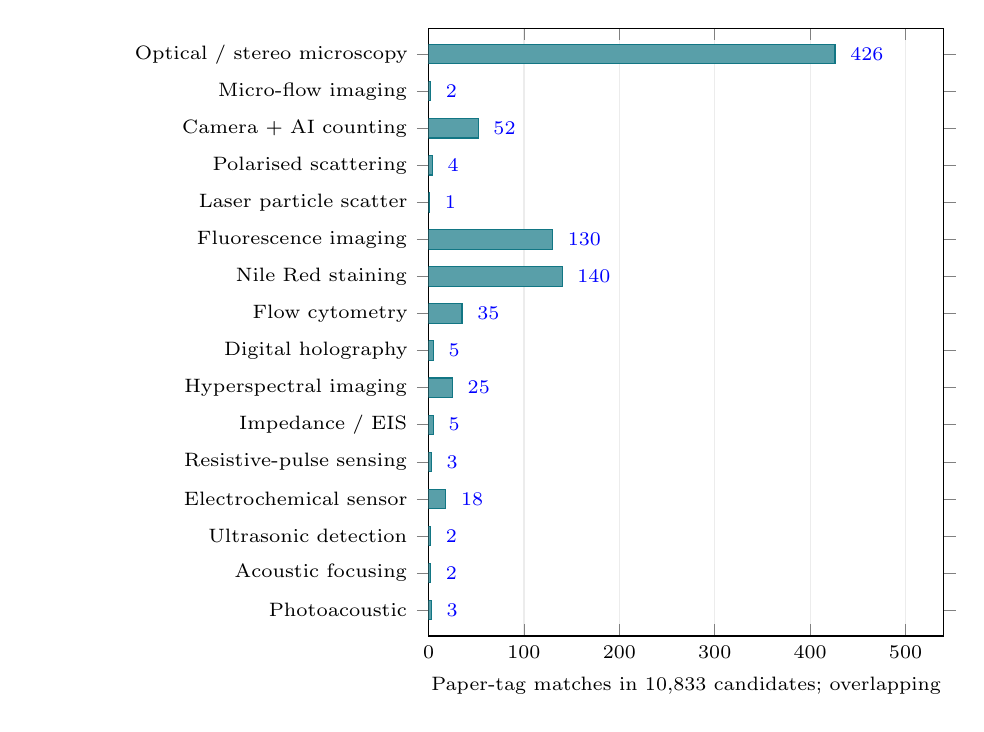
\begin{tikzpicture}
\begin{axis}[xbar,width=.67\linewidth,height=9.3cm,xmin=0,xmax=540,
 ymin=-.7,ymax=15.7,ytick={0,1,2,3,4,5,6,7,8,9,10,11,12,13,14,15},yticklabels={{Photoacoustic},{Acoustic focusing},{Ultrasonic detection},{Electrochemical sensor},{Resistive-pulse sensing},{Impedance / EIS},{Hyperspectral imaging},{Digital holography},{Flow cytometry},{Nile Red staining},{Fluorescence imaging},{Laser particle scatter},{Polarised scattering},{Camera + AI counting},{Micro-flow imaging},{Optical / stereo microscopy}},
 yticklabel style={font=\scriptsize,align=right,text width=4.7cm},tick label style={font=\scriptsize},
 xmajorgrids=true,grid style={gray!15},bar width=7pt,
 xlabel={Paper-tag matches in 10,833 candidates; overlapping},xlabel style={font=\scriptsize},
 nodes near coords,point meta=x,every node near coord/.append style={font=\scriptsize,anchor=west,xshift=2pt}]
\addplot+[draw=mpteal,fill=mpteal!70] coordinates {(426,15) (2,14) (52,13) (4,12) (1,11) (130,10) (140,9) (35,8) (5,7) (25,6) (5,5) (3,4) (18,3) (2,2) (2,1) (3,0)};
\end{axis}\end{tikzpicture}
\caption{Potential optical, electrical and acoustic particle-readout families; ultrasound sample preparation is intentionally excluded from the direct-detector chart.}\label{fig:expanded-sensing}
\end{figure}

\begin{figure}[H]\centering
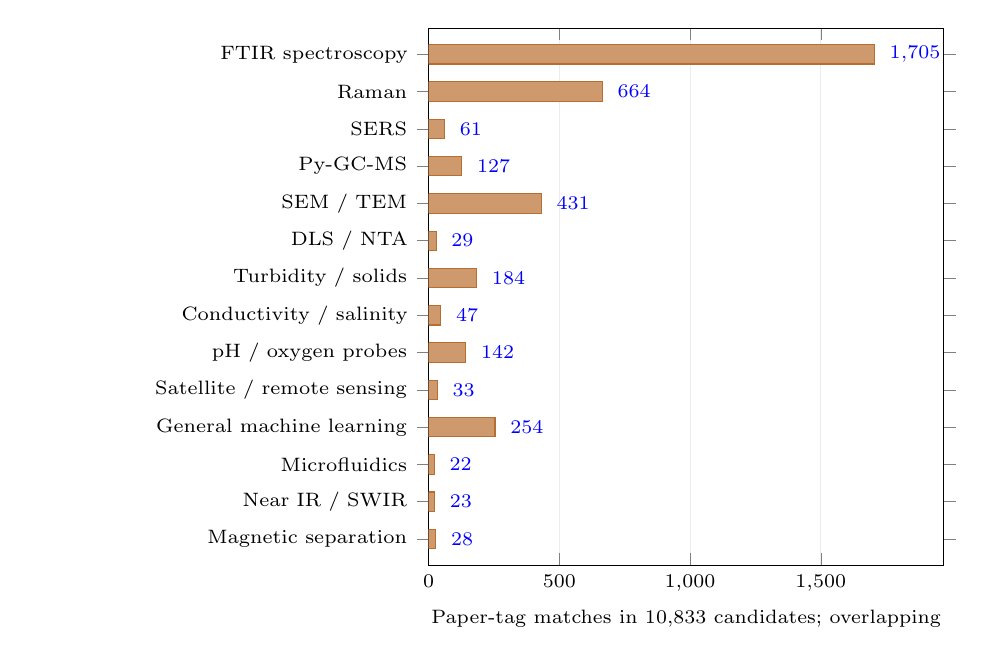
\begin{tikzpicture}
\begin{axis}[xbar,width=.67\linewidth,height=8.4cm,xmin=0,xmax=1970,
 ymin=-.7,ymax=13.7,ytick={0,1,2,3,4,5,6,7,8,9,10,11,12,13},yticklabels={{Magnetic separation},{Near IR / SWIR},{Microfluidics},{General machine learning},{Satellite / remote sensing},{pH / oxygen probes},{Conductivity / salinity},{Turbidity / solids},{DLS / NTA},{SEM / TEM},{Py-GC-MS},{SERS},{Raman},{FTIR spectroscopy}},
 yticklabel style={font=\scriptsize,align=right,text width=4.7cm},tick label style={font=\scriptsize},
 xmajorgrids=true,grid style={gray!15},bar width=7pt,
 xlabel={Paper-tag matches in 10,833 candidates; overlapping},xlabel style={font=\scriptsize},
 nodes near coords,point meta=x,every node near coord/.append style={font=\scriptsize,anchor=west,xshift=2pt}]
\addplot+[draw=mpgold,fill=mpgold!70] coordinates {(1705,13) (664,12) (61,11) (127,10) (431,9) (29,8) (184,7) (47,6) (142,5) (33,4) (254,3) (22,2) (23,1) (28,0)};
\end{axis}\end{tikzpicture}
\caption{Reference techniques, pretreatment, ancillary probes and model/mapping tools: prevalence of terms does not imply field sensing capability.}\label{fig:expanded-support}
\end{figure}


The first figure compares particle-readout technologies; the second shows reference, auxiliary and analysis terms. Together with the older broad 14-category figure, these distinguish \emph{literature prominence} from \emph{operational selection}. For example, FTIR and Raman tags are common because the techniques are useful for polymer identification, but routine bench spectroscopy fails the portable, rapid and low-infrastructure gate. Conversely, few impedance or flow-imaging mentions do not imply that they are unworkable; instead they signal a smaller and less mature direct evidence base \cite{Blevins2021,Lee2022,Kim2024,Warraich2025}.

\small
\begin{longtable}{@{}p{.8cm}p{6.0cm}rccp{5.4cm}@{}}
\caption{Expanded method identification across the original 10,833 papers. Matches are title/abstract/keyword terms, may overlap, and are not proof that the authors applied the method.}\label{tab:allmethods}\\
\toprule ID & Explicitly screened method family & Papers & A & B & Constraint / decision rationale \\\midrule
\endfirsthead
\multicolumn{6}{l}{\emph{Table continued: expanded method identification}}\\\toprule
ID & Method family & Papers & A & B & Main barrier \\\midrule
\endhead
\bottomrule\endfoot
\multicolumn{6}{l}{\textbf{Collection / pretreatment}}\\[2pt]
M01 & Manual field grab / surface sampling & 1,122 & S & P & volume/contamination control \\
M02 & Pump / automated water intake & 13 & S & S & flow calibration \& carry-over \\
M03 & Membrane / vacuum filtration & 107 & C & P & time \& membrane recovery \\
M04 & Density / flotation separation & 373 & X & C & reagents and waste \\
M05 & Chemical / enzymatic digestion & 113 & X & C & chemical safety/time \\
M06 & Ultrasonic sample sonication & 10 & X & C & preparation, not detection \\
M41 & Microfluidics / lab-on-chip handling & 22 & S & S & microchannels need antifouling/volume control \\
M46 & Magnetic / electrostatic separation & 28 & X & C & functionalisation / recovery controls \\
\multicolumn{6}{l}{\textbf{Optical particle readout}}\\[2pt]
M07 & Brightfield / stereo optical microscopy & 426 & C & P & particle appearance not polymer proof \\
M08 & Flow-through / micro-flow particle imaging & 2 & P & C & volume/focus \& duplicates \\
M09 & Camera + AI counting / segmentation & 52 & P & P & MP-like images vs true MPs \\
M10 & Polarised light scattering / polarimetry & 4 & C & C & sediment/algae discrimination \\
M11 & Laser / nephelometric particle scattering & 1 & C & C & optical non-specificity \\
M12 & Fluorescence / laser induced fluorescence & 130 & C & C & photobleaching/matrix \\
M13 & Nile Red fluorescent staining & 140 & X & C & wet chemistry, false positives \\
M14 & Flow cytometry / fluorescence cytometry & 35 & C & C & expensive/complex; identity uncertain \\
M15 & Digital holography / inline holography & 5 & C & C & optical alignment, inference \\
M16 & Hyperspectral / multispectral laboratory imaging & 25 & C & C & cost/illumination/background \\
M17 & UV-visible absorbance / colorimetry & 3 & S & S & matrix dependence \\
M47 & Smartphone / handheld digital microscopy & 0 & C & P & low cost; resolution and repeatability \\
M49 & Optical coherence tomography (OCT) & 1 & C & C & cost/penetration/selectivity \\
\multicolumn{6}{l}{\textbf{Electrical / acoustic}}\\[2pt]
M18 & Electrical impedance spectroscopy (EIS) & 5 & C & C & salt/electrode artefacts \\
M19 & Resistive pulse / Coulter / microchannel sensing & 3 & C & C & throughput/clogs, size cut-off \\
M20 & Electrochemical / voltammetric sensing & 18 & C & C & electrode specificity \& fouling \\
M21 & Dielectrophoresis / capacitive particle sensing & 73 & C & C & field geometry and salinity \\
M22 & Microwave / RF dielectric resonance & 1 & C & C & water permittivity dominates \\
M23 & Ultrasonic attenuation / scattering detection & 2 & C & C & particle/background contrast \\
M24 & Acoustic focusing / acoustophoresis & 2 & C & C & enrichment only, not counting \\
M25 & Photoacoustic sensing / spectroscopy & 3 & C & C & specialised transducers/lasers \\
M44 & Nanopore ionic current / pulse sensing & 0 & C & C & pore clogging; selectivity \\
M48 & QCM / piezoelectric mass sensor & 6 & C & C & selective adhesion / drift \\
\multicolumn{6}{l}{\textbf{Reference / analytical}}\\[2pt]
M26 & FTIR / micro-FTIR / ATR-FTIR & 1,705 & X & X & specialist instrument; useful external reference \\
M27 & Raman / micro-Raman spectroscopy & 664 & X & X & specialist instrument; useful external reference \\
M28 & Surface-enhanced Raman (SERS) & 61 & X & X & nanostructured substrates/laser \\
M29 & Py-GC-MS / thermal decomposition & 127 & X & X & polymer mass, destructive/lab \\
M30 & SEM / TEM electron microscopy & 431 & X & X & fixed equipment; morphology \\
M31 & Dynamic light scattering / nanoparticle tracking & 29 & X & X & nanoparticle proxy, no polymer proof \\
M32 & Plasmonics / SPR / LSPR sensing & 5 & C & C & substrates/selectivity/expense \\
M33 & Fluorescence tagging / immunoassay & 7 & X & C & reagents and field stability \\
M42 & NIR / SWIR / near infrared spectroscopy & 23 & C & C & spectral sampling \& water interference \\
M43 & Laser-induced breakdown spectroscopy (LIBS) & 7 & X & X & pulsed laser / target preparation \\
M45 & AFM atomic force microscopy & 20 & X & X & lab-scale nanoscale morphology \\
\multicolumn{6}{l}{\textbf{Indirect / geospatial}}\\[2pt]
M34 & Turbidity / suspended solids & 184 & S & S & not selective for MP \\
M35 & Conductivity / resistivity / salinity probe & 47 & S & S & ions dominate; auxiliary covariate \\
M36 & pH / dissolved oxygen / temperature probes & 142 & S & S & environmental covariates only \\
M37 & RGB / aerial drone imagery & 6 & S & S & water appearance, not individual MPs \\
M38 & Satellite / remote sensing / spectral indices & 33 & S & S & surface signal, calibration needed \\
M39 & GIS / geostatistics / spatial interpolation & 13 & S & S & maps points; not sensing \\
M40 & Machine learning / predictive regression & 254 & S & S & model does not independently establish polymer \\
\end{longtable}
ormalsize
\noindent\textbf{Legend:} \textbf{P} = preferred core candidate; \textbf{C} = conditional feasibility; \textbf{S} = supporting/enabling method, not a stand-alone MP counter; \textbf{X} = excluded as routine core under the no-specialist-lab constraint. These are \emph{engineering triage labels}, not published validation status.\par

\noindent\textbf{Audit trail.} The companion \texttt{data/Method\_to\_Paper\_Index.csv} identifies every term match by document, DOI and text excerpt. An additional \texttt{Unclassified\_Technical\_Leads.csv} records 137 unmatched candidates with potential instrumentation language, and the larger unmatched file retains the other candidates for reconsideration. These files are not exclusion decisions. Because rule boundaries differ from the earlier screen, the counts of broad categories and detailed categories must never be summed. The candidate pool may also contain methods outside the explicitly defined vocabulary: an unmatched paper is \emph{not} excluded from the literature review.

\clearpage
\subsection{Track A: retained candidates versus eliminated methods}
\begin{table}[H]\centering\footnotesize
\caption{First-pass decisions for Track A (live boat operation). Priority is conditional on controlled-sample tests.}\label{tab:Ascreen}
\begin{tabularx}{\linewidth}{@{}L{3.2cm}L{2.2cm}YY@{}}\toprule
\rowcolor{mpblue!12}\textbf{Method concept} & \textbf{Decision} & \textbf{Reason to retain or use} & \textbf{Why another method is not sufficient} \\\midrule
Flow-cell camera + AI \cite{Microflow2023,Lee2022,UrbanCNN2024} & \textbf{Core candidate} & Direct particle images, possible events/known observed volume, auditable frames. & Polymer identity unknown; requires de-duplication and good wet optics.\\
Polarised/laser scatter \cite{Polarized2021} & \textbf{Conditional} & Fast, compact optical signature; little sample handling. & Nonplastic solids, bubbles and changing optical matrix.\\
Impedance/EIS; resistive pulses \cite{Blevins2021,Kim2024,Warraich2025} & \textbf{Conditional} & Compact electronics and continuous-channel possibility. & Electrolyte changes/fouling; electrode chemistry differs from pulse counting.\\
Holography / flow cytometry \cite{Wang2024} & \textbf{Conditional} & More features than bulk turbidity; potential high-throughput. & Hardware/optics cost and particle-level truth remain challenging.\\
Acoustic concentration \cite{Ohori2025} & \textbf{Supporting only} & Upstream enrichment may help low concentrations. & Enrichment does not count or prove MP identity.\\
Turbidity, conductivity, RGB imagery \cite{MPWE00002,MPWE04211} & \textbf{Auxiliary only} & Cheap spatial covariates, interference monitoring, mapping context. & No inherent polymer specificity; must not be called MP particles/L without calibration.\\
FTIR, Raman, Py-GC-MS \cite{Sefiloglu2024} & \textbf{Eliminate onboard} & Strong offline reference value. & Specialist, slow and maintenance-intensive for an autonomous boat.\\
\bottomrule\end{tabularx}
\end{table}

\subsection{Track B: retained candidates versus eliminated methods}
\begin{table}[H]\centering\footnotesize
\caption{First-pass decisions for Track B (known-volume collection; portable shoreline processing).}\label{tab:Bscreen}
\begin{tabularx}{\linewidth}{@{}L{3.2cm}L{2.2cm}YY@{}}\toprule
\rowcolor{mpblue!12}\textbf{Method concept} & \textbf{Decision} & \textbf{Reason to retain or use} & \textbf{Limitation to check} \\\midrule
Measured-volume filtration + digital microscope / AI \cite{Lee2022,Ermolin2024,MPWE00012} & \textbf{Core candidate} & Inspect each sample and save images; repeat counts without boat motion. & Time per sample, contamination, particle losses and false plastic IDs.\\
Static camera + segmentation \cite{UrbanCNN2024} & \textbf{Core analysis stage} & Digitised audit trail and reduced labour. & Representative training set, blind human re-count and operator bias.\\
Nile Red fluorescence \cite{ErniCassola2017,Minor2023} & \textbf{Conditional} & Increases contrast for small suspected particles. & Dyes/waste and false positives; not obligatory without safe handling.\\
EIS, scattering and microfluidics \cite{Blevins2021,Warraich2025,Polarized2021} & \textbf{Conditional} & Portable bench-side alternative readouts. & May not outperform microscope counts without careful calibration.\\
Density separation / digestion \cite{Ermolin2024} & \textbf{Conditional preparation} & May reduce natural-particle background. & Reagents, time, recovery and safety; avoid unless justified.\\
FTIR / Raman / Py-GC-MS \cite{Sefiloglu2024} & \textbf{Eliminate routine shoreline} & Occasional external polymer confirmation, if possible. & Requires off-site specialist facility; not a deployable processing stage.\\
\bottomrule\end{tabularx}
\end{table}

\subsection{Transparent weighted comparison \emph{after} the hard gates}
The following scores are \textbf{illustrative engineering assumptions} on a 1--5 scale, not empirical rankings established by the papers. Six criteria are weighted differently for each workflow: validity of a particles/L output (A/B 30\%), portability (A 20\%, B 10\%), throughput (A 20\%, B 10\%), independence of specialist labs (A 12\%, B 20\%), robustness (A 10\%, B 15\%) and affordability (A 8\%, B 15\%). A higher number is better. The total is
\begin{equation}
S_{\mathrm{track}} = \sum_{k=1}^{6} w_{k,\mathrm{track}}\,q_k,\quad \sum_k w_k=1,\quad q_k\in\{1,2,3,4,5\}.
\end{equation}
A score never overrides a failed hard gate. For example, bulk conductivity may be inexpensive and fast, yet remains an auxiliary probe unless a transferably validated model establishes MP concentration. Conversely a micro-FTIR system may provide a strong analytical reference but is excluded from both \emph{routine deployment} tracks.

\footnotesize
\begin{longtable}{@{}p{4.05cm}ccrrp{5.45cm}@{}}
\caption{Illustrative track-weighted feasibility of candidate \emph{system concepts}; scores and gates are expert engineering assumptions, NOT study performance. Score range: 1--5.}\label{tab:weighted}\\
\toprule Concept & A gate & B gate & A / 5 & B / 5 & Basis / risk \\ \midrule
\endfirsthead
\toprule Concept & A & B & A / 5 & B / 5 & Basis / risk \\ \midrule
\endhead
\bottomrule\endfoot
Flow-through camera + AI & P & C & 3.62 & 3.60 & Pumped, measured flow; object recognition; count/volume \\
Portable filtration + microscope / AI & X & P & 3.60 & 3.80 & Collect known V; filter; visual count; optional AI \\
Micro-flow imaging particle analyser & C & C & 3.14 & 3.00 & Imaging and morphometry within flow cell \\
Polarised light scattering & C & C & 3.44 & 3.25 & Measure material-related polarisation/scattering contrast \\
Optical particle scattering / counter & C & C & 3.44 & 3.25 & Laser scatter pulses, particle-size proxy \\
Electrical impedance / EIS & C & C & 3.24 & 3.15 & Frequency-dependent electrical response \\
Resistive-pulse microfluidic & C & C & 3.14 & 3.00 & Particle-transit electrical pulses \\
Nile Red fluorescence + imaging & X & C & 2.70 & 2.75 & Controlled portable stain and microscope \\
Flow cytometry / fluorescence counting & C & C & 2.74 & 2.55 & Flow and laser fluorescence/scatter readout \\
Digital holographic particle imaging & C & C & 3.26 & 3.20 & Reconstruct digital holograms and size/categorise \\
Hyperspectral imaging & C & C & 2.34 & 2.35 & Multi-band optical signatures \\
Acoustic focusing + downstream counting & S & S & 2.44 & 2.50 & Enrich suspension; another sensor must count \\
Ultrasonic direct attenuation & C & C & 3.12 & 2.95 & Acoustic losses interpreted as particle-related \\
Electrochemical functionalised electrode & C & C & 2.64 & 2.60 & Electrode binding/redox response \\
Remote RGB / turbidity proxy & S & S & 3.40 & 3.20 & Predict MPs from surface colour/turbidity \\
Bulk conductivity / resistivity proxy & S & S & 3.40 & 3.20 & Predict MPs from ion-dependent water impedance \\
Micro-FTIR / micro-Raman & X & X & 2.50 & 2.65 & Polymer spectrum and particle ID \\
Py-GC-MS polymer mass & X & X & 2.20 & 2.35 & Destructive laboratory polymer mass quantification \\
SEM / TEM & X & X & 1.50 & 1.60 & Electron morphology imaging \\
\end{longtable}\normalsize


\subsection{Decisions carried into the prototype phase}
The first build should demonstrate \textbf{Track B: known-volume collection, controlled shoreline imaging and a GPS-linked provisional concentration map}; its low-infrastructure operation makes it a practical validation baseline. \textbf{Track A: flow-through camera/AI} is the main live candidate because it offers an interpretable path from particle image to event count. \textbf{EIS or resistive pulse} can be tested in parallel but advances only if blinded MP-vs-silt and salt-sensitivity experiments yield reliable discrimination. Polarised scattering and Nile Red remain options if they improve specificity without unacceptable overhead. This is a \emph{screening decision}, not a finding that any method already satisfies the stakeholder's true-MP validation requirement.

\subsection{Camera + AI: counting from collected or flowing water}
Lee \emph{et al.} developed skip-connection U-Net architectures for automated particle counting in microscopy images \cite{Lee2022}. Xu and Wang examined neural segmentation of urban-water MPs; these studies assess \emph{image segmentation}, not yet continuous MP particles/L accuracy on a boat \cite{UrbanCNN2024}. Choran and Ormeci investigated micro-flow imaging, including particle shape and size information in flowing samples, with bubble and matrix-related limitations \cite{Microflow2023}. A complementary flow-cytometry classification study highlights the possibility of discriminating natural particles using additional optical signatures and machine learning, at the cost of more elaborate instrumentation \cite{Wang2024}. These studies support the core concept of Track A and the image-analysis step of Track B, but they do not prove either full workflow meets the stakeholder target without further tests.

\subsection{Impedance/EIS: possible boat-mounted electrical alternative}
An electrode/flow-cell assembly applies an electrical excitation and measures a response; conventional EIS uses the complex frequency-dependent impedance $Z(f)=V(f)/I(f)$. A passing particle can perturb a confined measurement field, while dissolved salts, temperature and fouling can also dominate response. Blevins \emph{et al.} survey emerging approaches including impedance \cite{Blevins2021}. Kim \emph{et al.} used electrochemical/EIS measurements with specialised NiMoO$_4$ electrodes to detect PVC model MPs \cite{Kim2024}. Warraich \emph{et al.} studied a MXene-coated microfluidic \emph{resistance} sensor; a DC bridge is not the same as multifrequency EIS \cite{Warraich2025}. The electrical path is a \emph{research option} for Track A, but it offers no easy visual audit trail and requires rigorous salinity/particle challenge tests.

\subsection{Polarisation, fluorescence, filtration and sample concentration}
Polarised light-scattering responses have been investigated to discriminate model plastic particles from other particles, but turbidity and water matrix remain key issues \cite{Polarized2021}. Nile Red can highlight candidate MPs for camera analysis; stained organics and dye-handling logistics make it more suited to controlled shoreline post-processing than to a completely continuous, reagent-free boat sensor \cite{ErniCassola2017,Minor2023}. Portable filtration followed by digital microscopy is simpler but slow per sample and potentially vulnerable to contamination. Integrated microfluidic sample preparation has also been studied, although channel clogging and recovery remain concerns \cite{Zhang2023}. Acoustic focusing can enrich particles before a downstream detector, but enrichment alone does not identify the particles or establish the source concentration \cite{Ohori2025}.

\begin{table}[H]\centering\footnotesize
\caption{Methods selected from the candidate literature and where they fit the two workflows. \emph{Proposed fit} is an engineering judgement, not a demonstrated boat-ready product.}\label{tab:methods}
\begin{tabularx}{\linewidth}{@{}L{2.6cm}L{3.0cm}YY@{}}\toprule
\rowcolor{mpblue!12}\textbf{Method / citation} & \textbf{Principle and reported setting} & \textbf{Track A live boat} & \textbf{Track B shoreline} \\\midrule
Camera + U-Net \cite{Lee2022,UrbanCNN2024} & Image segmentation / particle counts from microscope images & Good AI basis; needs live flow cell, non-plastic rejection & \textbf{Very good}; image filtered/settled sample, audit individual detections \\
Micro-flow imaging \cite{Microflow2023} & Optical morphology from a flowing sample & \textbf{Good conceptual match}; optics/flow control & Useful but less essential than static microscopy \\
Nile Red + imaging \cite{ErniCassola2017,Minor2023} & Dye fluorescence enhances candidate particle contrast & Poor routine fit: reagent and waste handling & \textbf{Possible}; needs blanks, staining protocol, false-positive assessment \\
Impedance / EIS \cite{Blevins2021,Kim2024} & Electrical response to particles/interfaces & Possible experimental adjunct; high interference risk & Bench-test candidate, not needed for minimal Track B \\
Electrical microfluidics \cite{Warraich2025} & Particle-induced bridge signal in restricted channel & Potentially compact; clogging and salinity issues & Optional comparative sensor test \\
Polarised scattering \cite{Polarized2021} & Polarisation response from illuminated particles & Potential optical upgrade after camera baseline & Optional discrimination add-on \\
Filtration + portable microscopy \cite{Ermolin2024,MPWE00012} & Isolate/count imaged suspected particles from known volume & Hard to automate continuously & \textbf{Core portable reference}; membrane, blank, operator check \\
FTIR/Raman \cite{Sefiloglu2024,MPWE00012} & Spectral polymer identification & Not realistic as routine student boat payload & Not assumed available; occasional external confirmation desirable \\
Acoustic focusing \cite{Ohori2025} & Particle enrichment using acoustic force & Optional complex front-end & Possible but costly/complex compared with filtration \\
\bottomrule\end{tabularx}
\end{table}

\section{Direct comparison: strengths, weaknesses and technical risks}
\begin{table}[H]\centering\footnotesize
\caption{Trade-offs for the two deployment tracks. Advantages are conditional on successful validation.}\label{tab:proscons}
\begin{tabularx}{\linewidth}{@{}L{2.4cm}YY@{}}\toprule
\rowcolor{mpblue!12}\textbf{Criterion} & \textbf{Track A: live flow-cell measurement} & \textbf{Track B: collected sample + shore processing} \\\midrule
Main advantage & Near-continuous spatial coverage and immediate feedback; routes can be adapted & Easier to build, clean, inspect, re-count and troubleshoot; lower payload complexity \\
Main disadvantage & Optical flow stability, power draw, wet electronics, fouling and duplicate-frame counting & Delayed map; sampling is discrete; more hands-on processing \\
Typical sensors & Camera + light + flowmeter; optional polariser/EIS and water-quality probe & Portable microscope + filtration cassette + camera/AI; optional dye \\
Volume denominator & Must calibrate \emph{observed} fluid volume, not merely pump nominal throughput & Known collected volume; correct for subsampling and filter losses \\
Plastic specificity & Difficult in untreated turbid water; classifier may recognise natural fragments as plastic & Better visual access and optional stain, but still not spectroscopic polymer proof \\
Data integrity & Synchronise intake time, transit delay, frames, GPS and flow & Stable sample ID linked to GPS/time; track handling and filter IDs \\
Field practicality & More integrated engineering and maintenance risk & More achievable without lab access or expensive instrumentation \\
Map output & Updated continuously with QC; gaps where detector cannot perform & Heat map after batch processing; retain sampling points and extrapolation uncertainty \\
\bottomrule\end{tabularx}
\end{table}

% \subsection{Prototype choices consistent with the expanded elimination process}
% \begin{table}[H]\centering\footnotesize
% \caption{Prioritisation consistent with the explicit gate and weighted tables in Section~\ref{sec:formal_selection}. Engineering priorities are provisional, not published performance scores.}\label{tab:triage}
% \begin{tabularx}{\linewidth}{@{}L{3.0cm}L{2.2cm}YY@{}}\toprule
% \rowcolor{mpblue!12}\textbf{Concept} & \textbf{Priority} & \textbf{Why it is practical} & \textbf{Must demonstrate first} \\\midrule
% B: collection + portable microscope/AI & \textbf{First prototype} & Minimal optics on boat; samples and images can be rechecked & Spike recovery, non-plastic false positives, repeatable particles/L estimate \\
% A: pumped camera + AI flow cell & \textbf{Second prototype} & No return-to-shore delay; direct path to near-live map & Calibrated observed volume, focus, frame de-duplication, matrix robustness \\
% A: EIS / microfluidic electrical sensor & Feasibility side-test & Small possible footprint and fast electronics & MP discrimination across salinity, sediment, size; event count vs bulk response \\
% RGB turbidity / conductivity proxy & Auxiliary only & Cheap and easy to mount on boat & Out-of-sample correlation with verified MP count; uncertainty and confounder tests \\
% \bottomrule\end{tabularx}
% \end{table}

% \section{Validation without routine laboratory equipment}
% \subsection{The scientific boundary}
% The stakeholder still requires reliable estimates demonstrably related to actual MPs. A camera trained on shape alone counts \emph{MP-like particles}, and a conductivity sensor measures ionic electrical properties. Neither can prove polymer identity in an unknown environmental sample on its own. Therefore the team should separate three validation goals: \emph{(i)} count known test particles, \emph{(ii)} reject non-plastic interferents, and \emph{(iii)} establish polymer-specific credibility using occasional external standards/confirmation if at all available. If the third goal is not met, label the map ``estimated/suspected MP-like particle concentration'' rather than certified MP concentration \cite{Blevins2021,ErniCassola2017,Ermolin2024}.

% \subsection{Portable experiments the team can perform}
% \begin{table}[H]\centering\footnotesize
% \caption{Low-infrastructure validation plan suitable for bench, shoreline and boat trials; targets must be set experimentally.}\label{tab:verification}
% \begin{tabularx}{\linewidth}{@{}L{3.0cm}YY@{}}\toprule
% \rowcolor{mpblue!12}\textbf{Test} & \textbf{How to conduct it without specialist chemistry equipment} & \textbf{Required record / failure indicator} \\\midrule
% Blanks and contamination & Run filtered-water and empty-cassette controls; cover samples, use clean handling, record blank detections & Blank particle count and field contamination events \\
% Known-particle dilution & Prepare known-volume suspensions of characterised PE/PP/PS beads/fragments at several levels; repeat & Measured-vs-expected counts, bias, recovery, detection limits \\
% Non-plastic challenge & Independently add silt, algae and bubbles in MP-free water and mixed suspensions & False-positive/negative rates and how accuracy changes with water matrix \\
% Size, speed and volume & Vary particle sizes, pump speed, optical focus and sample volumes & Detectable size range, flow cell volume, repeat counting rate \\
% Independent image review & Blindly re-label a subset of raw images by human operators; repeat on different days & Precision/recall, disagreements, drift and repeatability \\
% Shoreline method agreement & Split paired field samples between Track A and Track B; compare blind outputs & Agreement, MAE/RMSE and location-specific errors \\
% External polymer spot-check (optional) & Send only a small stratified sample of recovered particles to a university/collaborator when feasible & Polymer-confirmation rate; record unavailable if not done \\
% \bottomrule\end{tabularx}
% \end{table}

For Track A, the denominator must correspond to \emph{fluid actually observed} by the image sensor: $\widehat{C}_{A}=N_{\mathrm{unique,classified}}/V_{\mathrm{imaged}}$. For Track B, $\widehat{C}_{B}=(N_{\mathrm{counted}}-N_{\mathrm{blank}})/(V_{\mathrm{collected}}\,r)$ only when a defensible recovery fraction $r$ is measured and the entire analysed fraction is accounted for. Until polymer specificity is validated, both concentrations are \emph{suspected MP-like counts per litre}. Blank correction and recovery uncertainty must not be silently assumed.

\subsection{Heat-map generation and communication}
The software takes $(\mathrm{lat},\mathrm{lon},t,V,N,\mathrm{QC})$ from either track, computes a concentration estimate and displays \emph{actual measured locations} before optional spatial interpolation. Each map needs a legend with units, a declared size cutoff, an explicit timestamp/survey period, sample density and unsupported areas. Interpolate only within supported coverage. Compare prediction values against a subset of \emph{withheld} sample stations; do not validate the interpolation using exactly the same stations on which it was fitted. Real-time maps and shore-processed maps should use the same schema so their performance can be compared directly.

% \section{Recommended next steps and decision milestones}
% \begin{enumerate}
% \item \textbf{Specify the measurand.} Set target size fraction and concentration units (particles/L, not area-normalised count unless explicitly justified). Choose whether the first prototype is for suspected MPs rather than polymer-certified MPs.
% \item \textbf{Pilot Track B first.} Build clean collection cassettes, sample IDs, measured-volume collection, portable image capture, simple AI/threshold counting and GPS-linked CSV/map output.
% \item \textbf{In parallel, prototype Track A optics.} Pump through a transparent chamber; evaluate video quality, one-particle/one-count tracking, tubing-delay correction and cleaning effort on the same known-particle dilutions.
% \item \textbf{Use EIS only as a gated side experiment.} Compare known MPs against salt, sediment and non-plastics; stop early if signals are dominated by water conductivity or unstable electrode effects.
% \item \textbf{Field trial both tracks.} Survey a modest route with replicated paired samples, contamination blanks and withheld locations; quantify device agreement and heat-map error.
% \item \textbf{Go/no-go decision.} Prefer Track A only if its extra automation produces trustworthy counts and repeatable operation; otherwise Track B can still satisfy the spatial-map objective through rapid shoreline post-processing. Seek limited independent polymer confirmation to support any claim of true MP concentration.
% \end{enumerate}

\section{Limitations of this working literature review}
The evidence base is a \emph{preliminary title/abstract candidate pool}. Automated categories overlap; a matched keyword does not establish experimental deployment, evidence quality or causal relationships. Selected cited papers illustrate operating principles and performance issues but are not a quantitative meta-analysis of all 10,833 papers. Detailed performance figures and protocols must be checked against full texts before a final thesis. The proposed tracks, tests and prioritisation are engineering recommendations motivated by the stakeholder brief and the reviewed candidate literature.

\printbibliography[title={References}]
\end{document}